\chapter{Adversarial Neural Network}
\label{chp:ANN}

In this chapter, the setup and training of the Adversarial Neural Network is described. The Network did not achieve the desired results in its initial configuration.
For this reason, different configurations for the implementation of the network structure are presented in addition to the hyper-parameter investigations.
In total three main approaches to the adversarial neural network were tested. The first one uses the understanding earned from training the classifier and the original approach introduced in the paper \enquote{Learning to pivot with Adversarial Networks}~\cite{Louppe:2016ylz}. The second approach uses the last hidden layer of the classifier as input for the adversary instead of using the output of the classifier. Lastly, the information of the hidden layer is compressed to a smaller layer before being transferred to the adversary.

The first section of the chapter focuses on the initial run of the ANN using the base network presented in chapter~\ref{chp:simpleNN}. The results are investigated and the hyper-parameters are adapted using an initial setup for the second network. The problems with this setup are explained and possible reasons are listed.
The second section describes the approach of using hidden layers as input. The results are compared to the initial approach and conclusions are drawn.
The third approach deals with further adapting the information from the hidden layer and is described in the third section.
Finally, the approaches are compared and possible further steps are listed.

\section*{Prerequisites}

The technical details for the setup are the same as for the classifying network as introduced in section~\ref{sec:technicals}.
The adversarial setup uses the classifier's general setup and architecture trained and tuned in chapter~\ref{chp:simpleNN} as a basis. For the classical setup, this output is used as input for the adversarial network.

In general, both the classifier and the adversary are pre-trained. That means they are trained on their tasks without using a combined loss-function to generate better starting conditions for the adversarial training iterations.
In addition, observing the losses of the networks during the pre-training indicates whether the networks influence each other.

\missingfigure{pre-training}



\section{Approach \RNum{1}: classical neural network}

As already stated, the initial setup uses the classifier as trained in chapter~\ref{chp:simpleNN} and an adversary inspired by this structure. Optimisation and activation remained the same while the architecture was simplified to factor the one-dimensional input into the system. Figure~\ref{fig:app1:classic} shows the results. The network response~\ref{fig:app1:classic:syst} has almost no signs of a separation. Furthermore, the systematic distribution seems to be more pushed to the background distribution which is completely opposite to the original goal. It hints that modifications to the setup should be made. While the loss for both networks decreases, no minimum that hinders the adversary from learning is found. The expected increase in adversarial loss does not occur. The early spike in the losses comes from the pretraining losses.

\begin{figure}[htbp]
    \centering
    \begin{subfigure}[b]{0.45\textwidth}
        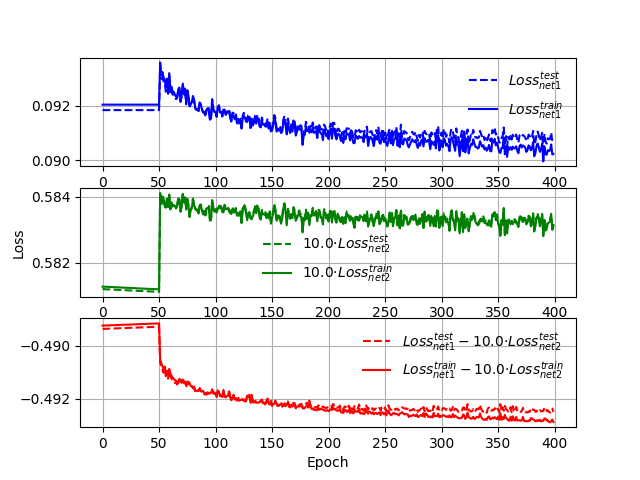
\includegraphics[width=\textwidth]{full_classic_losses}
        \caption{}
        \label{fig:app1:classic:losses}
    \end{subfigure}
\quad
    \begin{subfigure}[b]{0.45\textwidth}
        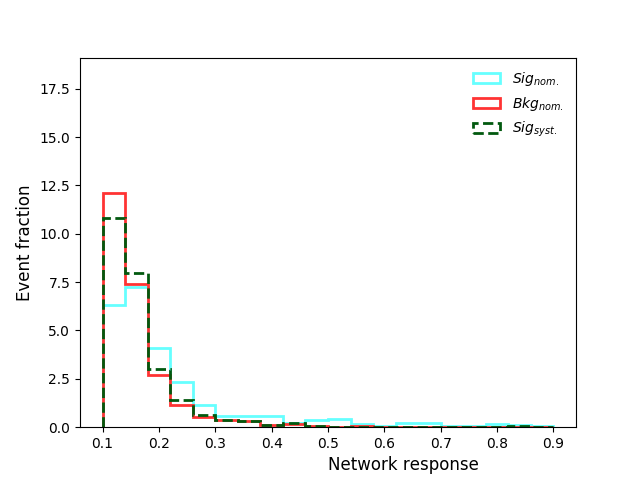
\includegraphics[width=\textwidth]{full_classic_syst}
        \caption{}
        \label{fig:app1:classic:syst}
    \end{subfigure}
    \caption[ANN results for a standard setup]{Results for an adversarial neural network using the classic approach and hyper-parameters adopted from the classifier. Figure~\subref{fig:app1:classic:losses} shows the losses; top to bottom: classifier, adversary, and combined loss. Figure~\subref{fig:app1:classic:syst} shows the separation for the nominal and the systematic sample; solid blue for nominal, dashed green for systematic, and red for the background.}
	\label{fig:app1:classic}
\end{figure}

It becomes clear that the optimised hyper-parameters for the classifier are not suitable for the task of training an adversarial neural network. This is an important insight because it means that the adversary is not something one can just add to a model to improve its sensitivity to a nuisance parameter. Instead, it is an integral aspect of a whole training procedure of its own. The next step taken during the analysis, presented here, is to try to investigate further what the performance of the combined network is strongly correlated with and how to understand what the network suffers from.

A hyper-parameter scan was performed in order to achieve a better performance for the adversarial neural network setup. The results for a very low learning rate and a non-existing momentum are shown in figure~\ref{fig:app1:half}.
With a slow optimisation the training becomes more stable and both networks can learn. This is assumed to be due that in an adversarial training, not just a minimum is sought. Instead, the classifier is first moved close to a minimum and then supposed to stay close to that model of decent classification, while also slowly adapting to features less sensitive to the systematic uncertainty. At some point, the adversarial loss stops decreasing. However, it does not increase again and in the response a difference between nominal and systematic sample is visible

As even with these updated hyper-parameters no model is found that is sufficiently independent on systematics, another change to the network has been elaborated.
On their own both networks improve their performance but in combination the classifier does not find a model that significantly downgrades the performance of the adversary.
The worst case scenario is that this is due to no such model existing. It is very well possible that for this particular task there is no training that is independent of systematics.
A simple change would be the set of input parameters. However, this would cause a whole new training problem and a subsequent hyper-parameter optimisation. For that reason, the input of the adversary was looked into. At this point, the adversary is just fed the sigmoid-output of the single, final node of the classifier. As mentioned earlier the amount of variables and the complexity of the architecture should be scaled with the task. Possibly the single output is sufficient to see a systematic dependency but not to improve the model using this insight. Furthermore, given the separation between \tW and \ttbar is small and the systematic to be minimised is their interference term, the classifier network's output may not be enough for both networks to find an insensitive minimum. Approach \RNum{2} is based on this thought.

\begin{figure}[htbp]
    \centering
    \begin{subfigure}[b]{0.45\textwidth}
        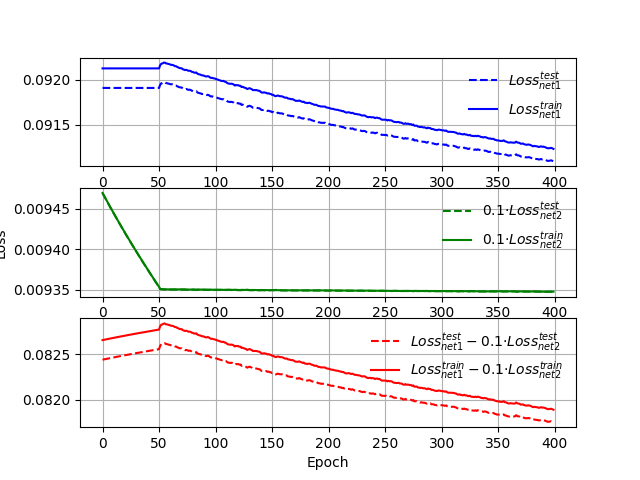
\includegraphics[width=\textwidth]{half_classic_losses}
        \caption{}
        \label{fig:app1:half:losses}
    \end{subfigure}
\quad
    \begin{subfigure}[b]{0.45\textwidth}
        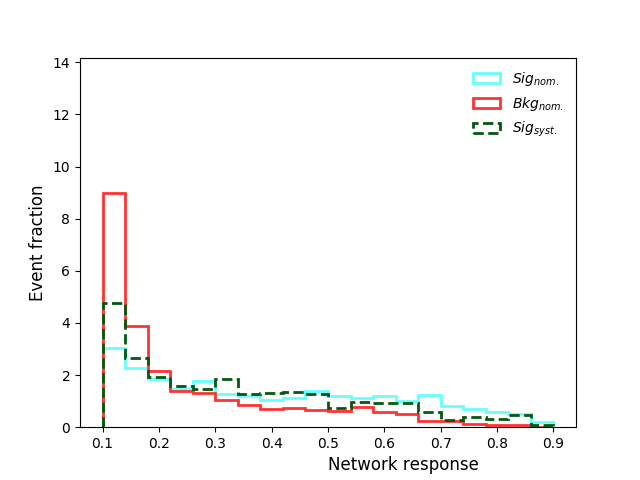
\includegraphics[width=\textwidth]{half_classic_syst}
        \caption{}
        \label{fig:app1:half:syst}
    \end{subfigure}
    \caption[ANN results for optimised parameters]{Results for an adversarial neural network using low learning rate and no momentum for the classifier. Figure~\subref{fig:app1:half:losses} shows the losses; top to bottom: classifier, adversary, and combined loss. Figure~\subref{fig:app1:half:syst} shows the separation for the nominal and the systematic sample; solid blue for nominal, dashed green for systematic, and red for the background.}
	\label{fig:app1:half}
\end{figure}


\section{Approach \RNum{2}: hidden layer input}

The amount of information given to the adversary is the output of one single node. This does not justify the usage of complex architecture and it allows no insight into the deeper dependencies of the classification model. Alternatively one can use the last hidden layer of the classifier which can be described as the final model the sigmoid-decision is based on. This is not fully correct as all dependencies of the model created in the last step are excluded this way. Nevertheless, it is a viable approximation worth testing.
This approach simply inputs the last hidden layer into the adversary without changing any other hyper-parameters. A hyper-parameter scan is then performed to test the behaviour of the network.
%
\begin{figure}[htbp]
    \centering
    \begin{subfigure}[b]{0.45\textwidth}
        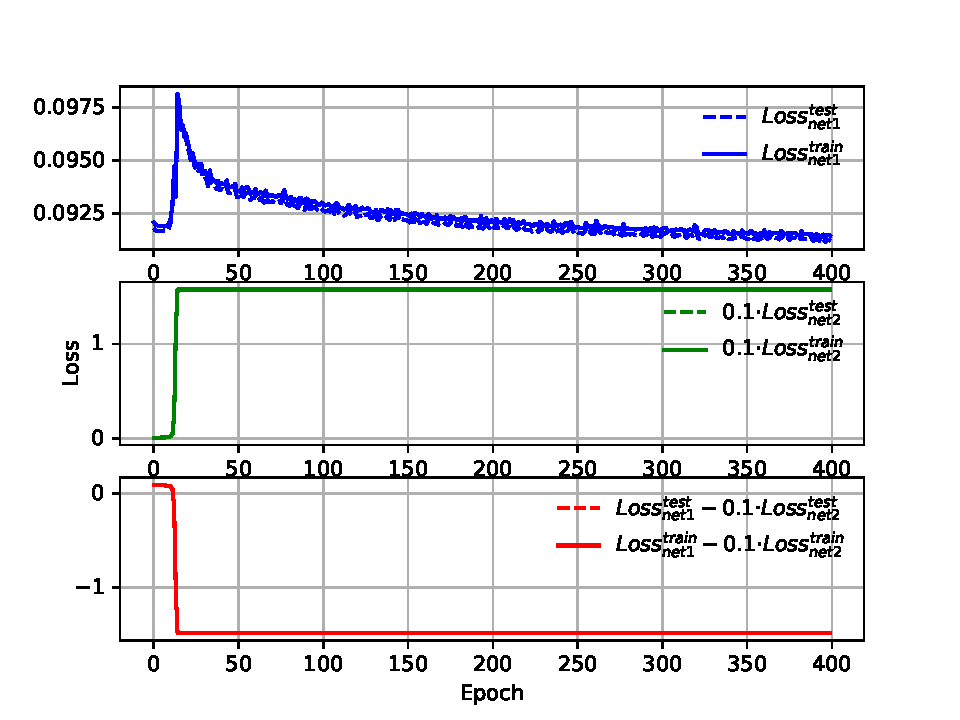
\includegraphics[width=\textwidth]{app2_losses2}
        \caption{Losses}
        \label{fig:app2:losses}
    \end{subfigure}
\quad
    \begin{subfigure}[b]{0.45\textwidth}
        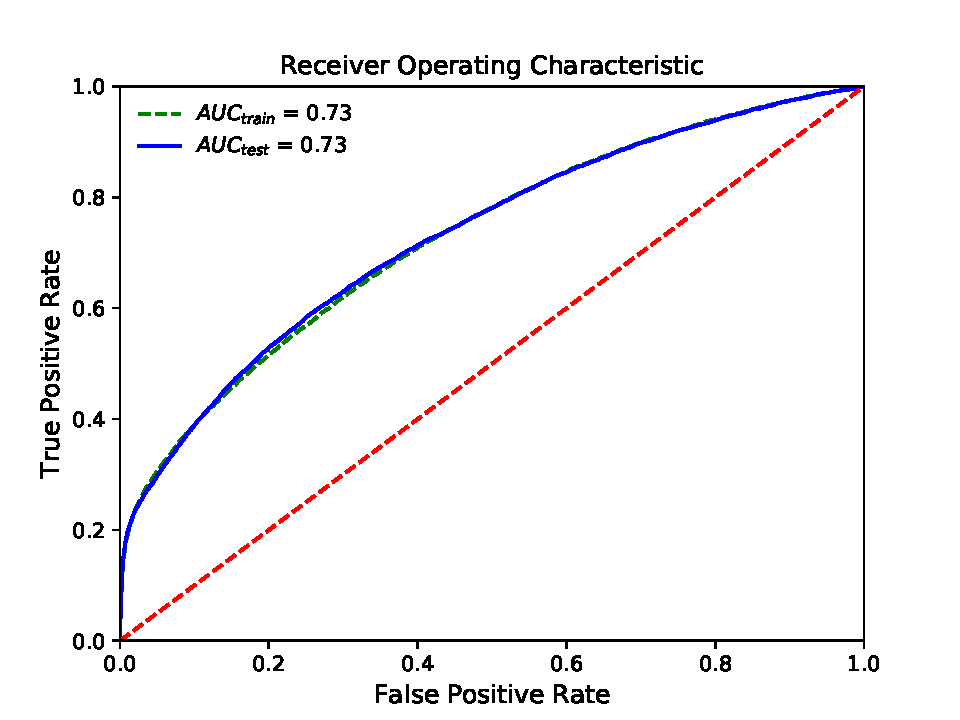
\includegraphics[width=\textwidth]{app2_ROC}
        \caption{ROC-curve}
        \label{fig:app2:ROC}
    \end{subfigure}

    \begin{subfigure}[b]{0.45\textwidth}
		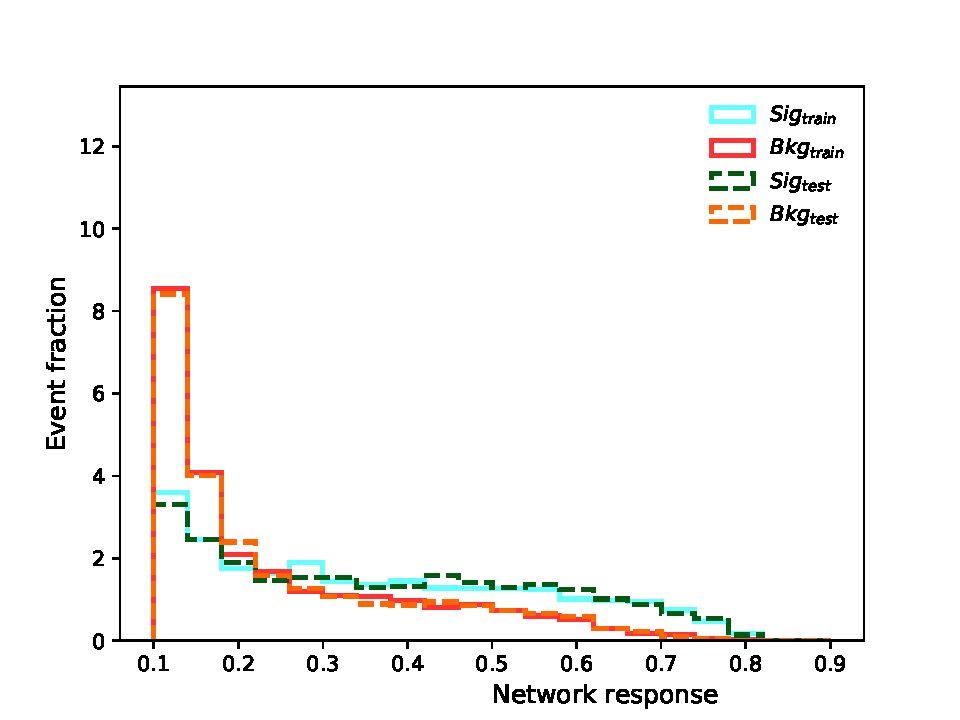
\includegraphics[width=\textwidth]{app2_sepa}
		\caption{Separation}
		\label{fig:app2:sepa}
	\end{subfigure}
\quad
	\begin{subfigure}[b]{0.45\textwidth}
		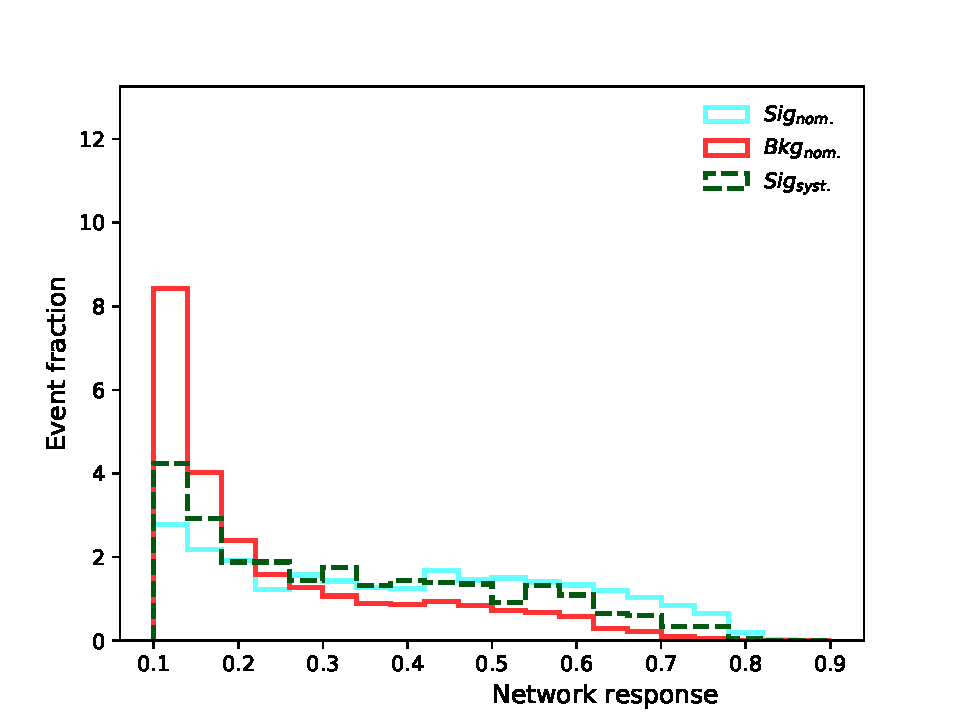
\includegraphics[width=\textwidth]{app2_syst}
		\caption{Systematic-Sensitivity}
		\label{fig:app2:syst}
	\end{subfigure}
    \caption[ANN results approach \RNum{2}]{Performance plots for the second approach. Both a slightly better separation and a lower sensitivity are visible.}
	\label{fig:app2}
\end{figure}
%
%
Using this setup the losses behave as desired. Figure~\ref{fig:app2} summarises the results. At one point the adversary fails to gain any information while the classifier keeps on learning and the combined loss decreases. The rise of the adversary's loss looks very steep but this is only a problem of the scale. In hindsight the model is very unstable and for many hyper-parameter setups it just stops working properly. Furthermore, the sensitivity to systematic samples does visibly improve. The improvements are small but the overall shape of the nominal and systematics distribution have become more alike and systematic distribution is less stretched to the background.
A further interesting behaviour was achieved for a relatively high learning rate of \num{0.2}. In this case the loss of the adversary increases later. The curve and separation is shown in figure~\ref{fig:app2:highlr}. After the usual 400 training epochs the model seems to still be changing. There is a possibility that a better model for a higher epoch count could be achieved using this setup. It also shows that the optimisation of the hyperparameters has significantly different effects depending on which approach is chosen.

\begin{figure}[htbp]
    \centering
    \begin{subfigure}[b]{0.45\textwidth}
        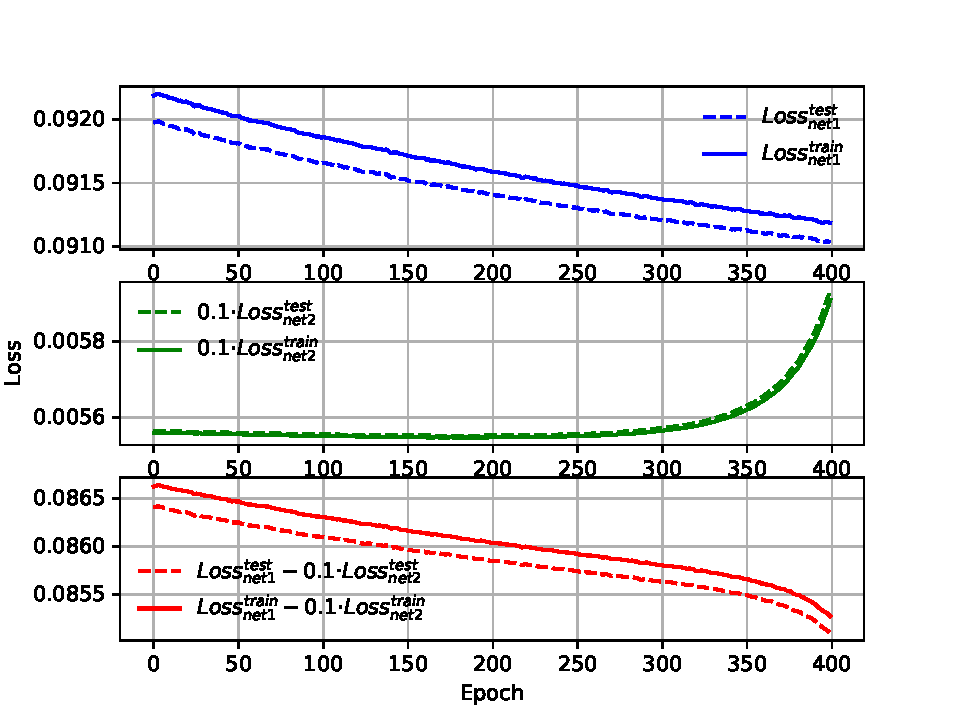
\includegraphics[width=\textwidth]{app2_highlr_losses}
        \caption{Loss}
        \label{fig:app2:highlr:losses}
    \end{subfigure}
\quad
    \begin{subfigure}[b]{0.45\textwidth}
        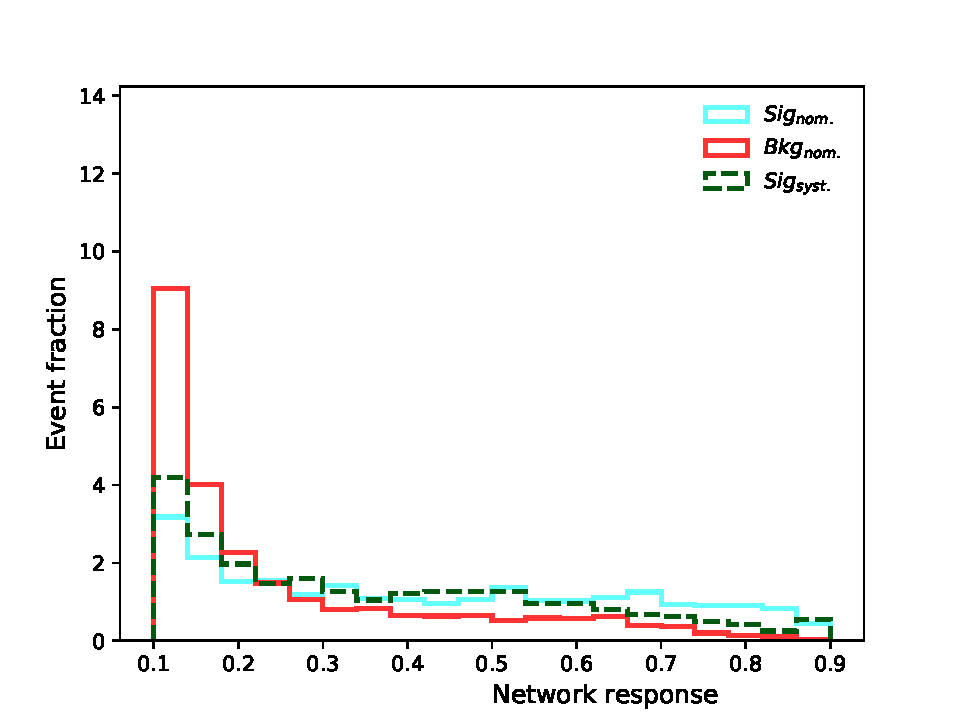
\includegraphics[width=\textwidth]{app2_highlr_syst}
        \caption{Separation of systematic and nominal in the response.}
        \label{fig:app2:highlr:syst}
    \end{subfigure}
    \caption[ANN approach \RNum{2}, high learning rate]{Behaviour of approach \RNum{2} for a learning rate of \num{0.2} showing a loss behaviour that could motivate a deeper analysis.}
	\label{fig:app2:highlr}
\end{figure}

\section{Approach \RNum{3}: compressed hidden layer input}

After using only a single input node in the classical approach and \num{128} nodes in the second approach, an intermediate number of inputs is tested. For approach \RNum{3}, a second to last layer with only \num{16} nodes is added to the classifier and then fed into the adversary. This way the input dimension is closer to the dimension of the classifier. In addition, it promises to control the instability of the second approach.

Parallel to the other approaches, a hyper-parameter scan was performed.
Figure~\ref{fig:app3} shows the result for an effective setup. The setup is about as unstable as that of approach \RNum{2}. Loss curves for different learning rates are shown in figure~\ref{fig:app3:misc}. The learning rate of \num{0.06} as originally used for the classifier performed badly for the classical, adversarial approach. For approach \RNum{3} it behaves different and in the end of the desired behaviour is visible. This is a feature that deserves more research. Furthermore figure~\ref{fig:app3:down:losses} diagrams the odd behaviour for the usually very good learning rate of \num{0.001}. 

\begin{figure}[htbp]
    \centering
    \begin{subfigure}[b]{0.45\textwidth}
        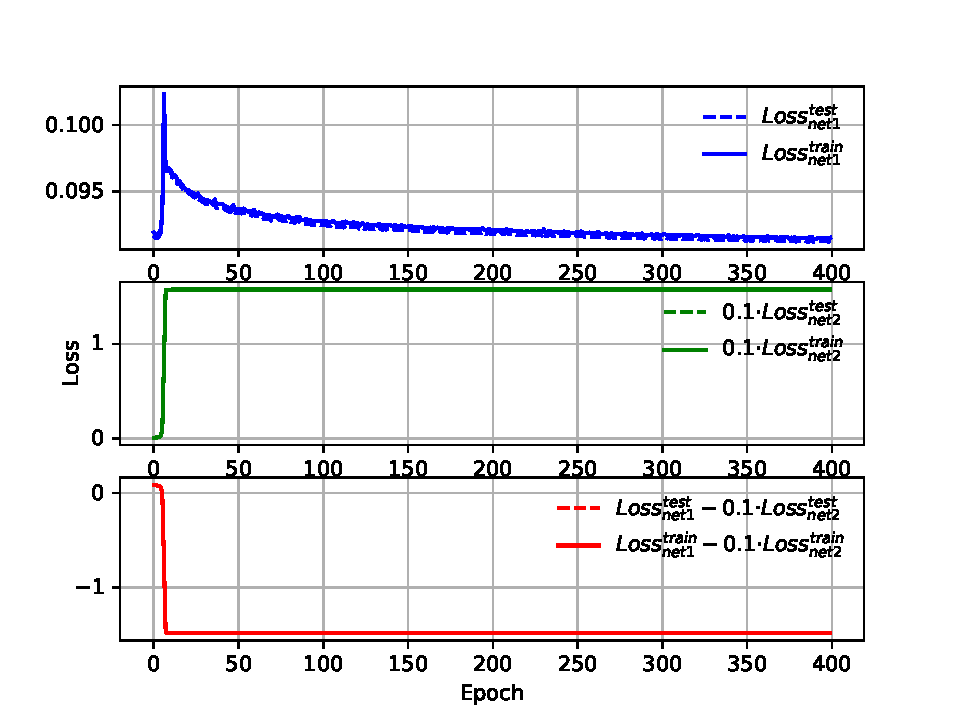
\includegraphics[width=\textwidth]{app3_losses2}
        \caption{Loss-curves}
        \label{fig:app3:losses}
    \end{subfigure}
\quad
    \begin{subfigure}[b]{0.45\textwidth}
        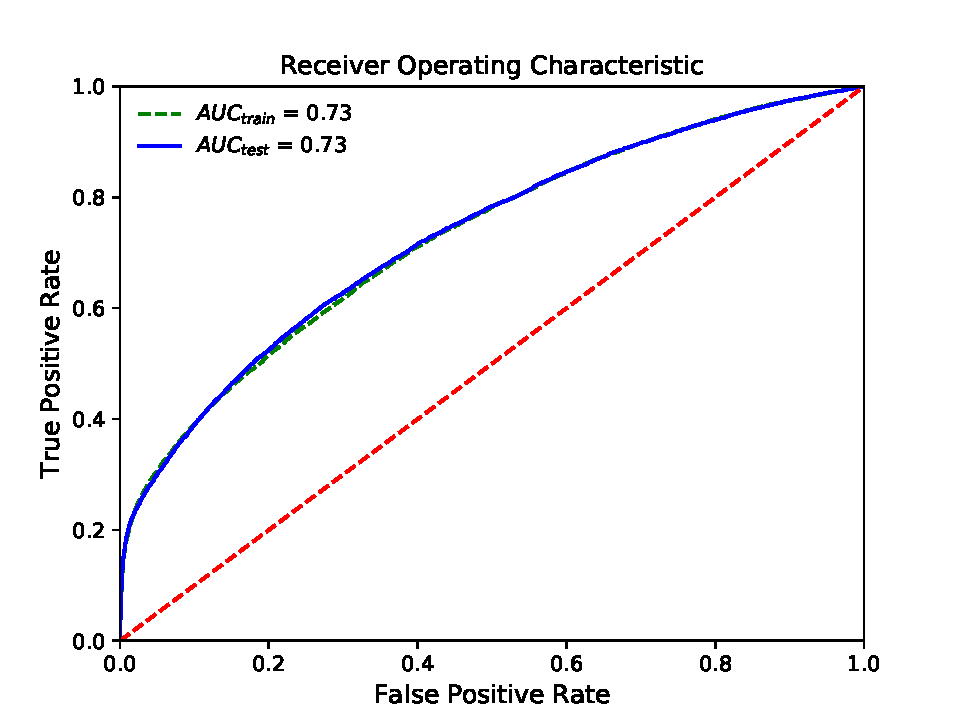
\includegraphics[width=\textwidth]{app3_ROC}
        \caption{ROC-curve}
        \label{fig:app3:ROC}
    \end{subfigure}

    \begin{subfigure}[b]{0.45\textwidth}
		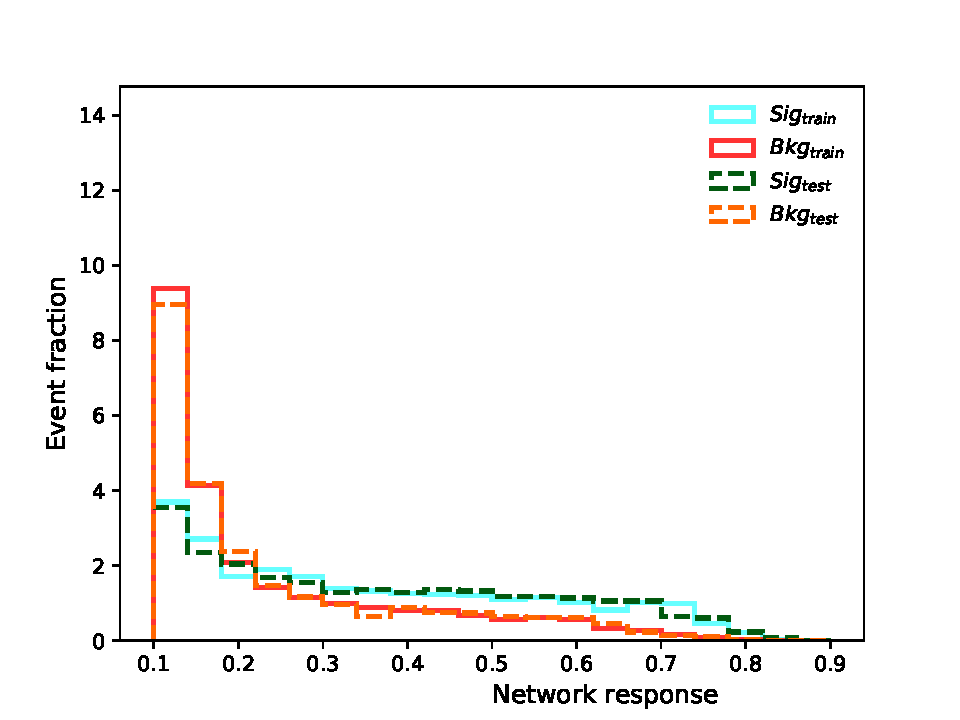
\includegraphics[width=\textwidth]{app3_sepa}
		\caption{Separation}
		\label{fig:app3:sepa}
	\end{subfigure}
\quad
	\begin{subfigure}[b]{0.45\textwidth}
		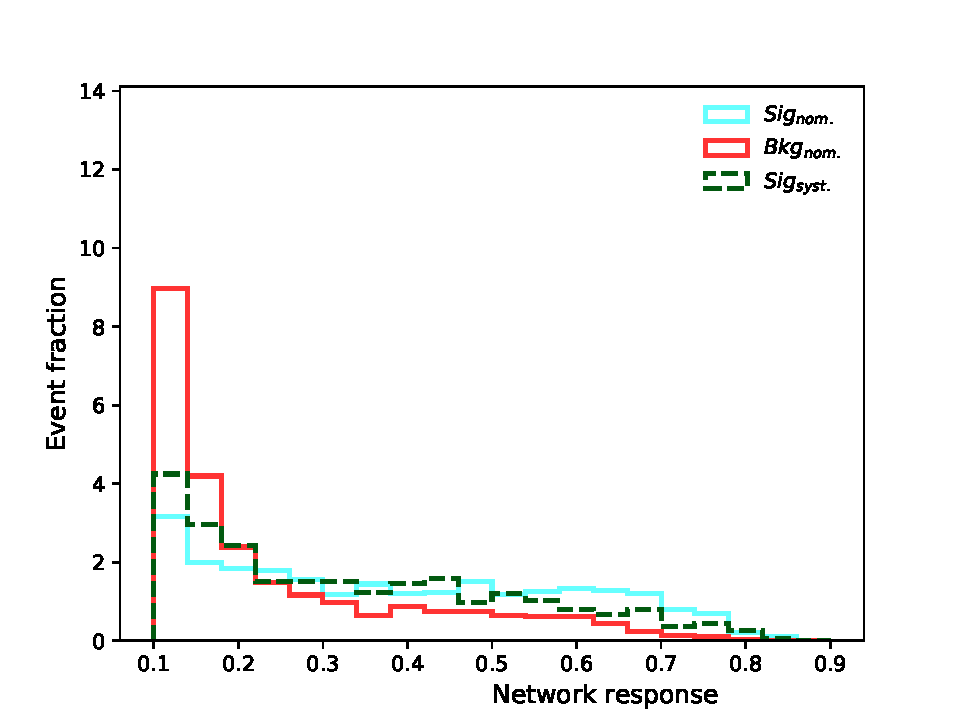
\includegraphics[width=\textwidth]{app3_syst}
		\caption{Systematic sensitivity}
		\label{fig:app3:syst}
	\end{subfigure}
    \caption[ANN results approach \RNum{3}]{Performance of approach \RNum{3}. The plots show no significant improvements. The losses behave as expected.}
	\label{fig:app3}
\end{figure}

\begin{figure}[htbp]
    \centering
    \begin{subfigure}[b]{0.45\textwidth}
        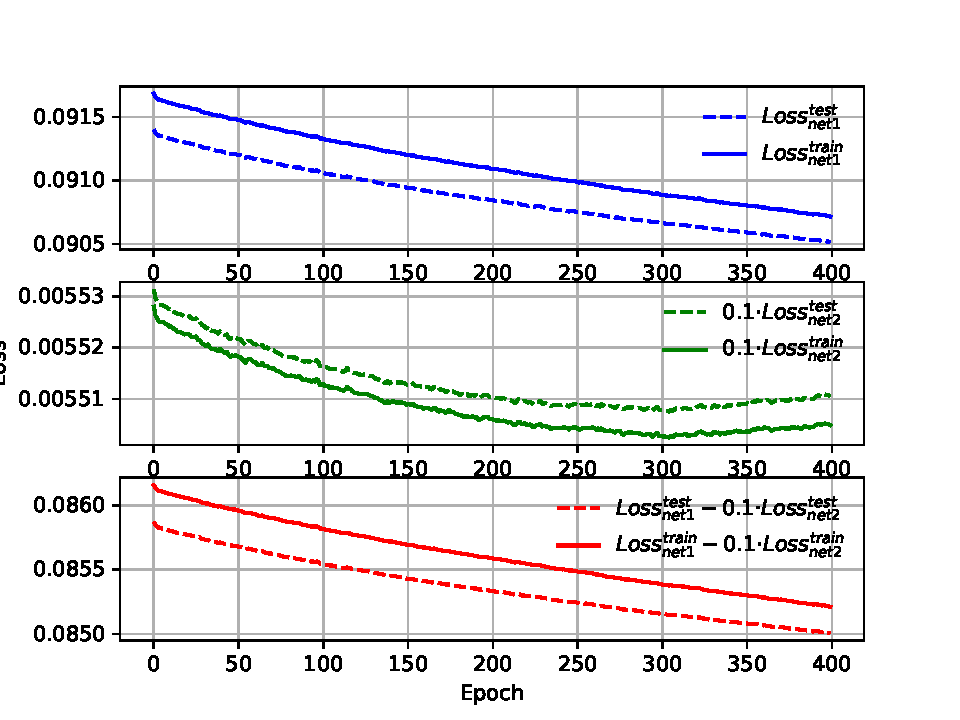
\includegraphics[width=\textwidth]{app3_classiclr_losses}
        \caption{}
        \label{fig:app3:classiclr:losses}
    \end{subfigure}
\quad
    \begin{subfigure}[b]{0.45\textwidth}
        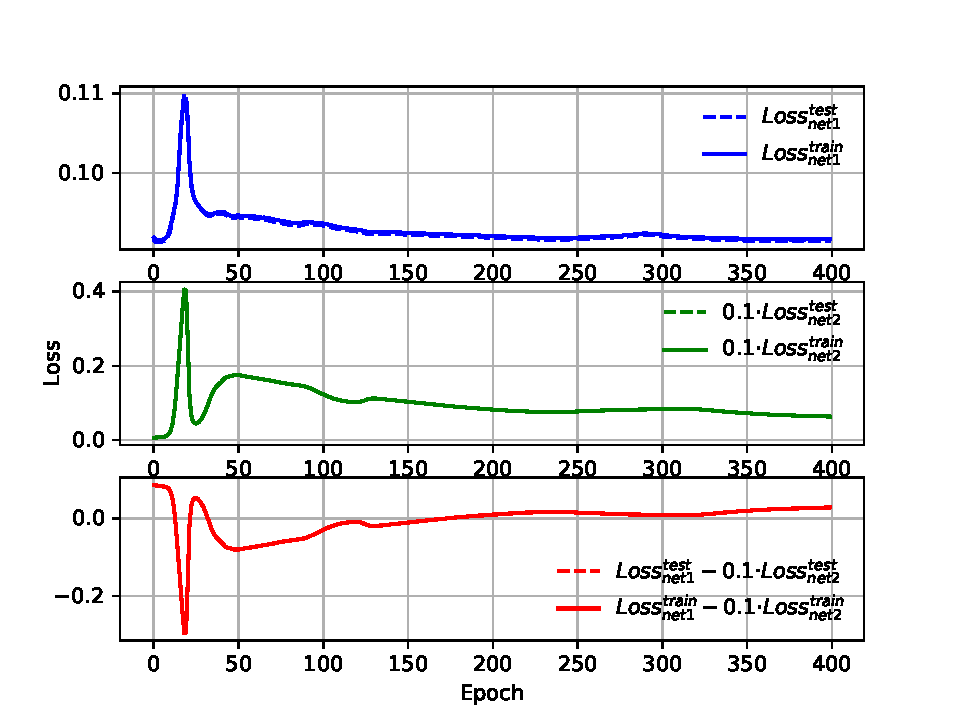
\includegraphics[width=\textwidth]{app3_down_losses}
        \caption{}
        \label{fig:app3:down:losses}
    \end{subfigure}
    \caption[Misc plots approach \RNum{3}]{Miscellaneous loss plots for approach \RNum{3}. Figure~\ref{fig:app3:classiclr:losses} shows the losses for a learning rate of \num{0.06} and figure~\ref{fig:app3:down:losses} for \num{0.001}.}
	\label{fig:app3:misc}
\end{figure}
\section{Summary}

In conclusion, the approach for an adversarial neural network to reduce a model's sensitivity on systematic uncertainties, as suggested in the paper \enquote{Learning to pivot with Adversarial Networks}~\cite{Louppe:2016ylz}, has not been successful at achieving the promised results for a \tW-\ttbar-separation. It was, however, possible to show the desired behaviour of the two adversarial networks. It has been shown that the input to the adversary is essential and a part of the analysis that would deserve more research. Furthermore, the adversarial neural network has proven to be a structure of its own rather than just two arbitrary classifiers combined. They have to be built around an unhurried optimisation process allowing both networks to slowly learn from different areas of the system's topology.
